\documentclass[12pt,letterpaper,english]{article}
\usepackage[T1]{fontenc}
\usepackage[latin9]{inputenc}
\pagestyle{empty}
\usepackage{amsmath}
\usepackage{amssymb}
\usepackage{graphicx}
\usepackage{bm}
\usepackage{multicol}
\usepackage{enumitem}

\usepackage{hyperref}
\hypersetup{
    colorlinks=true,
    linkcolor=blue,
    filecolor=magenta,      
    urlcolor=cyan,
}

\newcommand{\norm}[1]{\lVert#1\rVert}

\makeatletter

\special{papersize=\the\paperwidth,\the\paperheight}



\textwidth6.5in\textheight9in\topmargin-.25in\oddsidemargin0in\evensidemargin0in\parskip5pt\parindent0pt


\usepackage{fancyhdr}
\pagestyle{fancy}
\lhead{Reconfigurable Mechanical Vibrations Laboratory Kit}
\rhead{}


\usepackage{lastpage}
 
  
\rfoot{Page \thepage \hspace{1pt} of \pageref{LastPage}}

%\rfoot{\small }
\lfoot{Mechanical Vibrations: Lab 5}
\cfoot{}



\usepackage{babel}


\makeatother

\usepackage{babel}
\begin{document}
\global\long\def\Re{{\rm {Re }}}
 \global\long\def\cL{{\cal L}}
 \global\long\def\sq{{\rm {sq}}}
 \global\long\def\bfx{{\bf x}}
 \global\long\def\bfi{{\bf i}}
 \global\long\def\bfj{{\bf j}}


\begin{center}
\textbf{\large Lab Assignment 5: Continuous Systems}
\par\end{center}{\large \par}

The goal of this demo will be to investigate the resonant modes of a tensioned string under harmonic forcing. We will explore how the resonant frequencies are related to the string's tension and length. First, read through section E4 (``String-Wave Assembly'') in the Assembly Guide in order to set up the system.
\begin{center}
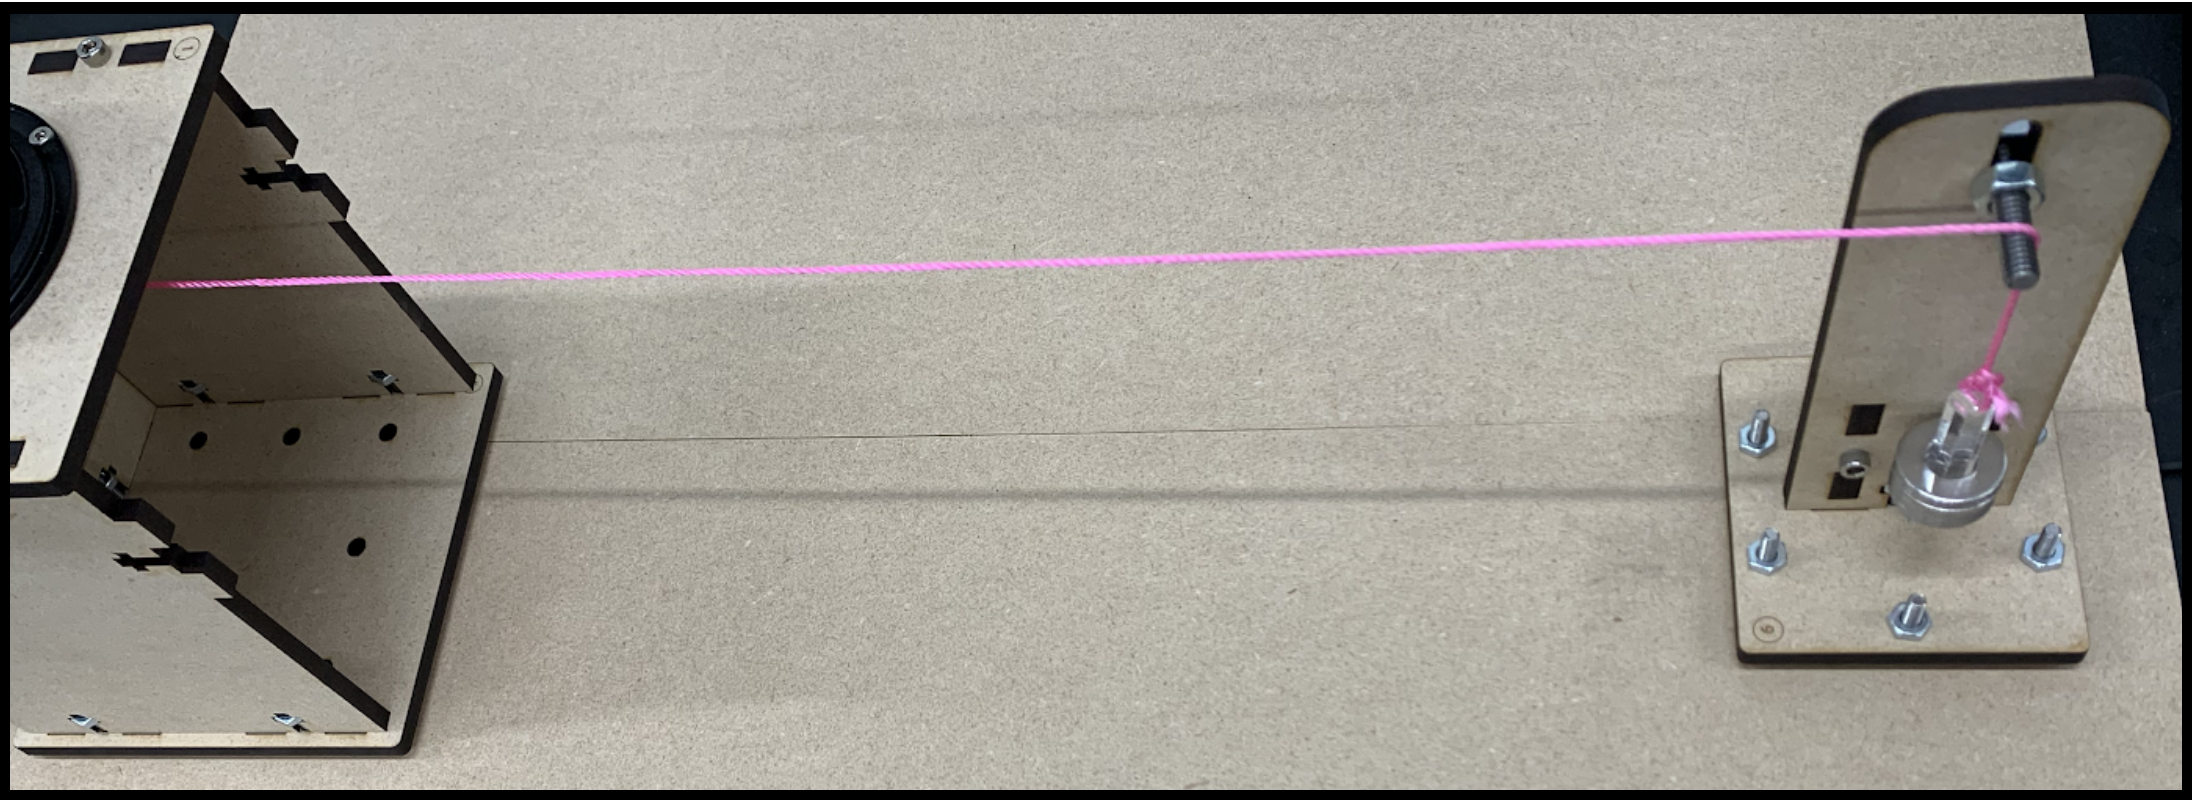
\includegraphics[width=5in]{lab5.png}
\end{center}

Cut the string into a longer section and a shorter section. We recommend that the `long' string be smaller or equal to approximately an arms length ($\sim$60cm) and the `short' string be around 30-40cm for good results.  Place the LED lights at the center of the string for strobing.

 %(this is to ensure that the fundamental mode is at least 20Hz, the minimum frequency at which the vibration of the speaker is reasonably uniform).  

\begin{enumerate}
\item To model this system, we will assume the string of length $L$ is under a constant tension $T$ that has constant linear density $\rho$.  In class, we saw that this physical system can be modeled by the PDE
\begin{equation}
\frac{\partial^2 u}{\partial t^2} = \frac{T}{\rho}\frac{\partial^2 u}{\partial x^2}. \nonumber
\end{equation}
In our lab, one end is shaken harmonically with amplitude $u(x=0,t)=a \cos{\omega t}$, and the other end is held fixed such that $u(x=L,t)=0$.  In the steps below we will seek the steady-state solution to the problem, ignoring any transients, and interpret the solution.

\begin{enumerate}
\item Since the problem is undamped and linear, we first make a guess of the steady-state solution of the form: $u(x,t)=f(x)\cos{\omega t}$.  By substituting our guess into the governing PDE, find an ODE for $f(x)$.  Solve the ODE and construct the form of $u(x,t)$.  You should still have two undetermined variables at this point.
\item Using appropriate boundary conditions, solve for the undetermined coefficients to find the steady-state solution for $u(x,t)$.  Plot the amplitude of the response as a function of the driving frequency $\omega$.
\item Using your expression for the steady-state solution, find the frequencies at which the amplitude is predicted to diverge (e.g. the resonant frequencies).  Compare your result to the natural frequencies of the equivalent free problem solved in class.
\item Reinterpret your result from the prior part in terms of the timescales in the problem. 

{\it \small Hint: Recall that we can interpret $c=\sqrt{T/\rho}$ as a wave speed in this problem.  First compute the time it takes for a wave to travel the length $L$ of the string.}
\end{enumerate}
\item Move on to the experiment.  Mount the longer string on the setup and place a total of 10 washers on the T-piece. Measure (approximately) the length of the string starting from the base of the shaker to the contact point with the screw at the string mount. We will investigate how the tension in the string affects the frequency at which each resonance occurs. If you are finding the string mount to be unstable, you can try taping it down or adding additional weight to its base.
\begin{enumerate}
\item Sweep through frequencies starting at around 10Hz (if the length is around an arms length), and identify the frequencies at which you experimentally observe the first 3 harmonic modes.  Sketch each of the modes and label them with their experimental natural frequency.
\item Repeat the same test but this time change the tension of the string by either adding weights (you can add some of the 3/8'' nuts) or removing some washers. Note that you want to change the mass by at least roughly $\sim$15g to most clearly observe the effects of changing tension.  Once again sweep through a range of frequencies to identify the frequencies at which the first 3 resonant modes occur.
\item The mass of one washer is 2.75g, while the mass of the T-piece is 2.6g. Use the expressions derived in the first part of this problem to predict the ratio of the original fundamental resonant frequency (10 washers) and the new fundamental resonant frequency (after having changed the mass). Then, calculate the ratio between the corresponding values that were determined experimentally and compare to your theoretical prediction. 

{\small \it Note: You may find it easier to identify the second resonant mode as compared to the fundamental mode. As such, you can alternatively predict and measure the ratios using this second mode instead.}
% Also note that during intermediate regimes, you will notice a combination of several harmonics, this is a good way to determine where the different modes are. Another way is to note at what frequency the modes clearly transition and to use that as a guide.
\end{enumerate}
\item Next, switch the mounted string to the shorter piece and place a total of 10 washers on the T-piece. Measure (approximately) the length of the string starting from the base of the shaker to the contact point. 
\begin{enumerate}
\item Repeat the frequency sweep to determine the approximate frequencies for the first 3 resonant modes. 
\item Next, based on the measured lengths of each string, calculate the ratio between the old fundamental frequency (long string) and the new fundamental frequency (short string). Then, calculate this ratio from the experimentally determined values. Compare the results.
\end{enumerate}

\item For any of the configurations described above, take a single still photograph of each resonant modes you can observe.  Combine these into a single image to include with your assignment.  No calculations are required for this part.

\item Provide feedback or ideas (positive and/or areas for improvement) on the setup process and continuous system lab.

\end{enumerate}

\end{document}
